%%%% ijcai15.tex

\typeout{IJCAI-15 Instructions for Authors}

% These are the instructions for authors for IJCAI-15.
% They are the same as the ones for IJCAI-11 with superficical wording
%   changes only.

\documentclass{article}
% The file ijcai15.sty is the style file for IJCAI-15 (same as ijcai07.sty).
\usepackage{ijcai15}

% Use the postscript times font!
\usepackage{times}

\usepackage{helvet}
\usepackage{courier}
\usepackage{bm}
\usepackage{amsmath}
\usepackage{cases}
\usepackage{multirow}
\usepackage{algorithm}
\usepackage{algorithmic}
\usepackage{booktabs}
\usepackage{graphicx}

\title{ A tri-factor matrix factorization method for drug target interaction prediction.\thanks{ some thanks.}}
\author{Dongliang Wu \\
Fudan University\\
Shanghai, China \\
xxx@xxx.edu.cn}

\begin{document}

\maketitle

\begin{abstract}
  Abstract.
\end{abstract}

\section{Introduction}
\indent In this paper, we proposed a novel framework to combine multiple similarity matrices in one model that improves prediction accuracy by taking advantages of both latent factor approaches and multi-similarities. Our contributions are summarized as follows:
\begin{itemize}
\item To incorporate the similarity of drugs(targets) for DTI prediction more effectively, we developed a tri-factor matrix factorization method to approximate similarity matrices. 
\item We provide a new way to combine multiple similarities with missing values.
\item We empirically show that our model outperforms other state-of-the-art methods on real world datasets.
\end{itemize}

\section{Method}
\subsection{Notation and Problem Setting}
First we briefly formalize the problem of drug-target interaction(DTI) prediction. Given a drug target interaction network $\bm{G}$, a set of drugs $\bm{D}=\{d_1,d_2,\cdots,d_{N_d}\}$ and a set of targets $\bm{T}=\{t_1,t_2,\cdots,t_{N_t}\}$, we can construct a DTI matrix $\bm{Y}$. Here $\bm{Y}$ is an $N_t\times N_d$ binary matrix whose rows and columns represent targets and drugs respectively. If drug $d_i$ and target $t_j$ interact with each other, then $\bm{Y}_{ij}$ = 1, else $\bm{Y}_{ij}$ = 0. \\
\indent Let $\{\bm{S}_d^1,\bm{S}_d^2,\cdots,\bm{S}_d^{M_d}\}$ be a set of drug similarity matrices, where each is a $N_d\times N_d$ matrix, and ${M_d}$ is the number of drug similarity matrices. $\bm{S_d}^{k_d}(i,j)$ is the similarity score between drug $d_i$ and drug $d_j$ in the $k$-th drug similarity matrix. Similarly let $\{\bm{S}_t^1,\bm{S}_t^2,\cdots,\bm{S}_t^{M_t}\}$ be a set of target similarity matrices, where each is a $N_t\times N_t$ matrix, and ${M_t}$ is the number of drug similarity matrices. $\bm{S_t}^{k_t}(i,j)$ is the similarity score between target $t_i$ and target $t_j$ in the $k$-th target similarity matrix. \\
\indent Let $\bm{\hat{Y}}$ be a score matrix, where the $(i,j)$-element of $\bm{\hat{Y}}$, i.e. $\bm{\hat{Y}}(i,j)$, shows the score that drug $d_i$ and target $t_j$ interact with each other. The objective of this article is to estimate $\bm{\hat{Y}}$ so that $\bm{\hat{Y}}$ should be consistent with $\bm{Y}$.

\subsection{Multiple Similarities Tri-factor Matrix Factorization (MSTMF)}
We first introduce a state-of-the-art matrix factorization model as our basic. Given a drug-target interaction matrix $\bm{Y}_{N_t\times N_d}$, a general framework of matrix factorization is:
\begin{equation}
(\bm{P},\bm{Q})=\mathop{\arg\min}_{\bm{P},\bm{Q}}\|\bm{H}\odot(\bm{Y}-\bm{P}\bm{Q}^T)\|_F^2
\end{equation}
where $\bm{P}\in\bm{R}^{N_t\times k}$ and $\bm{Q}\in\bm{R}^{N_d\times k}$, corresponding to feature spaces of targets and drugs, respectively. $\bm{T}$ is a $N_t\times N_d$ matrix, in which $\bm{H}_{ij}=1$ if $\bm{Y}_{ij}$ is a known drug-target pair( has interaction with each other or not); otherwise $\bm{H}_{ij}=0$. $\bm{H} \odot \bm{Z}$ denotes the element-wise product of matrices $\bm{H}$ and $\bm{Z}$. By estimating $\bm{P}$ and $\bm{Q}$, we can reconstruct $\bm{Y}$ so that unknown drug-target pairs have prediction scores.\\
\indent On the basis of above, we can plus a few more information into the framework. Suppose we have two similarity matrices, $\bm{S_t}$ for targets and $\bm{S_d}$ for drugs. A simple trying is leting the inner product of two drug feature vectors to approximate the corresponding similarity of two drugs ( $\bm{S_d}\approx\bm{Q}\bm{Q}^T$ ) and this is also the case with target similarity ( $\bm{S_t}\approx\bm{P}\bm{P}^T$ ).(Our previous work\cite{zheng2013collaborative}) \\
\indent However, this is not a good enough method to capture the correlation between two feature vectors. Because the correlation between two vectors maybe much more complex. On the other hand, this method is too restrictive to $\bm{P}$ and $\bm{Q}$ so that $\bm{\hat{Y}}=\bm{P}\bm{Q}^T$ may give poor predictions. So we add extra factors $\bm{W_d}$ and $\bm{W_t}$ to absorb the different scales of $\bm{S_d}, \bm{S_t}, \bm{P}, \bm{Q}, \bm{Y}$. I.e. let $\bm{S_d}\approx\bm{Q}\bm{W_d}\bm{Q}^T$, and $\bm{S_t}\approx\bm{P}\bm{W_t}\bm{P}^T$.\cite{tang2013exploiting} So $\bm{W_d}$($\bm{W_t}$) captures the drug feature(target feature) correlation. For multiple similarities, we can factorize them separately using different $\bm{W_d}$ or $\bm{W_t}$. \\
\indent Thus put all above together, we can write out the entire loss function:  \\
\begin{equation} % Loss function
\begin{split}
\mathcal{L} &= \|\bm{H}\odot(\bm{Y}-\bm{P}\bm{Q}^T)\|_F^2 \\
&+ \sum_{k_t=1}^{M_t}\|\bm{H_t}^{k_t}\odot(\bm{S_t}^{k_t}-\bm{P}\bm{W_t}^{k_t}\bm{P}^T)\|_F^2 \\
&+ \sum_{k_d=1}^{M_d}\|\bm{H_d}^{k_d}\odot(\bm{S_d}^{k_d}-\bm{Q}\bm{W_d}^{k_d}\bm{Q}^T)\|_F^2 \\
&+ \lambda(\|\bm{P}\|_F^2+\|\bm{Q}\|_F^2+\sum_{k_t=1}^{M_t}\|\bm{W_t}^{k_t}\|_F^2+\sum_{k_d=1}^{M_d}\|\bm{W_d}^{k_d}\|_F^2)
\end{split}
\end{equation}
where $\bm{H_t}^{(\cdot)}, \bm{H_d}^{(\cdot)}$ are introduced to handle missing values of some similarity matrices, and $\lambda$($\cdot$) is the regularization term. The parameters can be learned by minimizing the above loss function by using gradient descent algorithm. We write out the gradient and update rule directly below. The detailed algorithm is shown in Algorithm 1.\\
%temp use ---------------------------------------------------
\begin{equation} % Loss function
\begin{split}
\mathcal{L} &= \|\bm{H}\odot(\bm{Y}-\bm{P}\bm{Q}^T)\|_F^2 \\
&+ \lambda_t\sum_{k_t=1}^{M_t}\|\bm{H_t}^{k_t}\odot(\bm{S_t}^{k_t}-\bm{P}\bm{W_t}^{k_t}\bm{P}^T)\|_F^2 \\
&+ \lambda_d\sum_{k_d=1}^{M_d}\|\bm{H_d}^{k_d}\odot(\bm{S_d}^{k_d}-\bm{Q}\bm{W_d}^{k_d}\bm{Q}^T)\|_F^2 \\
&+ \lambda_l(\|\bm{P}\|_F^2+\|\bm{Q}\|_F^2+\sum_{k_t=1}^{M_t}\|\bm{W_t}^{k_t}\|_F^2+\sum_{k_d=1}^{M_d}\|\bm{W_d}^{k_d}\|_F^2)
\end{split}
\end{equation}
%------------------------------------------------------------

\textit{Gradient:}
\begin{equation} % gradient P
\begin{split}
\frac {\partial \mathcal{L}}{\partial \bm{P}} &=\bm{H}\odot(\bm{Y}-\bm{P}\bm{Q}^T)\bm{Q}\cdot(-1)\\
&+ \sum_{k_t=1}^{M_t} \Bigl[ \Bigl( \bm{H_t}^{k_t}\odot(\bm{S_t}^{k_t}-\bm{P}\bm{W_t}^{k_t}\bm{P}^T )\Bigr)^T\bm{P}\bm{W_t}^{k_t}\cdot(-1)\\
&+ \bm{H_t}^{k_t}\odot(\bm{S_t}^{k_t}-\bm{P}\bm{W_t}^{k_t}\bm{P}^T)\bm{P}(\bm{W_t}^{k_t})^T\cdot(-1) \Bigr]\\
&+ \lambda \bm{P}\\
\end{split}
\end{equation}
\begin{equation} % gradient Q
\begin{split}
\frac {\partial \mathcal{L}}{\partial \bm{Q}} &=\bm{H}\odot(\bm{Y}-\bm{P}\bm{Q}^T)\bm{P}\cdot(-1)\\
&+ \sum_{k_d=1}^{M_d} \Bigl[ \Bigl( \bm{H_d}^{k_d}\odot( \bm{S_d}^{k_d}-\bm{Q}\bm{W_d}^{k_d}\bm{Q}^T )\Bigr)^T\bm{Q}\bm{W_d}^{k_d}\cdot(-1)\\
&+ \bm{H_d}^{k_d}\odot(\bm{S_d}^{k_d}-\bm{Q}\bm{W_d}^{k_d}\bm{Q}^T)\bm{Q}(\bm{W_d}^{k_d})^T\cdot(-1) \Bigr]\\
&+ \lambda \bm{Q}\\
\end{split}
\end{equation}
\begin{equation} % gradient Wt^i
\begin{split}
\frac {\partial \mathcal{L}}{\partial \bm{W_t}^{k_t}} &=\bm{P}^T(\bm{S_t}^{k_t}-\bm{P}\bm{W_t}^{k_t}\bm{P}^T)\bm{P}\cdot(-1)+\lambda \bm{W_t}^{k_t}\\
 (k_t &= 1,\cdots,M_t)
\end{split}
\end{equation}
\begin{equation} % gradient Wd^j
\begin{split}
\frac {\partial \mathcal{L}}{\partial \bm{W_d}^{k_d}} &=\bm{Q}^T(\bm{S_d}^{k_d}-\bm{Q}\bm{W_d}^{k_d}\bm{Q}^T)\bm{Q}\cdot(-1)+\lambda \bm{W_d}^{k_d}\\
 (k_d &= 1,\cdots,M_d)
\end{split}
\end{equation}


\textit{Update Rule}:
\begin{equation}\label{update1} % update rule 
\begin{split}
\bm{P} &= \bm{P} - \eta\cdot\frac{\partial \mathcal{L}}{\partial \bm{P}}\\
\bm{Q} &= \bm{Q} - \eta\cdot\frac{\partial \mathcal{L}}{\partial \bm{Q}}\\
\bm{W_t}^{k_t} &= \bm{W_t}^{k_t} - \eta\cdot\frac{\partial \mathcal{L}}{\partial \bm{W_t}^{k_t}}\\ (k_t &= 1,\cdots,M_t) \\
\bm{W_d}^{k_d} &= \bm{W_d}^{k_d} - \eta\cdot\frac{\partial \mathcal{L}}{\partial \bm{W_d}^{k_d}}\\ (k_d &= 1,\cdots,M_d) \\
\end{split}
\end{equation}
%-------------algorithm
\renewcommand{\algorithmicrequire}{\textbf{Input:}}  %Use Input in the format of Algorithm
\renewcommand{\algorithmicensure}{\textbf{Output:}}  %Use Output in the format of Algorithm
\begin{algorithm}[htb] 
\caption{ the algorithm of MSTMF } 
\label{alg:Framwork} 
\begin{algorithmic}[1] 
\REQUIRE ~~\\ %Input
drug-target interaction matrix $\bm{Y}$;\\
target similarity matrices, $\{\bm{S}_t^1,\bm{S}_t^2,\cdots,\bm{S}_t^{M_t}\}$; \\
drug similarity matrices, $\{\bm{S}_d^1,\bm{S}_d^2,\cdots,\bm{S}_d^{M_d}\}$; \\
the number of latent factors , $K$;\\
weight matrix, $\bm{H}$, $\bm{H_t}^{k_t}$, $\bm{H_d}^{k_d}$; \\
(${k_t}=1,\cdots, M_t, {k_d}=1,\cdots, M_d$)\\
learning rate, $\eta$;\\

\STATE Initialize $\bm{P}$, $\bm{Q}$, $\bm{W_t}^{k_t}$, $\bm{W_d}^{k_d}$ randomly;\\
(${k_t}=1,\cdots, M_t, {k_d}=1,\cdots, M_d$)\\
\REPEAT 
\STATE Update $\bm{P}$, $\bm{Q}$, $\bm{W_t}^{k_t} $, $\bm{W_d}^{k_d} $  using Eq.(\ref{update1}); 
\UNTIL Stopping criterion is met;
\ENSURE ~~\\ %Output
predicted interaction matrix $\bm{\hat{Y}}=\bm{P}\bm{Q}^T$; %
\end{algorithmic}
\end{algorithm}

\subsection{Multiple Similarities Tri-factor Matrix Factorization With Weight (MSTMF-Weight)}
Last section we introduced a method of combining multiple similarities to predict drug-target interaction. In this section, we propose another kind of method. As we can see,  different similarity matrices provide different aspects of discriptions of similarities. And all similarity values are in the interval of [0,1]. So we combined the multiple similarity matrices linearly and acquired an unique similarity matrix as follows:
\begin{equation}
\begin{split}
\bm{S_t}&=\sum_{k_t=1}^{M_t}\alpha_{k_t}\bm{S_t}^{k_t}\quad( \bm{S_d}=\sum_{k_d=1}^{M_d}\beta_{k_d}\bm{S_d}^{k_d}) \\
&s.t. \sum_{k_t=1}^{M_t}\alpha_{k_t}=1\quad (\sum_{k_d=1}^{M_d}\beta_{k_d}=1)
\end{split}
\end{equation}
where $\alpha_{k_t}$ ($\beta_{k_d}$) is the weight of $k_t$-th ($k_d$-th) similarity matrix for targets (drugs). \cite{zheng2013collaborative} \\
Thus the objective function can be written as follow:
\begin{equation} % Loss function
\begin{split}
\mathcal{L} &= \|\bm{H}\odot(\bm{Y}-\bm{P}\bm{Q}^T)\|_F^2 \\
&+\|(\sum_{k_t=1}^{M_t}\alpha_{k_t}\bm{S_t}^{k_t}-\bm{PW_t}\bm{P}^T)\|_F^2 \\
&+\|(\sum_{k_d=1}^{M_d}\beta_{k_d}\bm{S_d}^{k_d}-\bm{QW_d}\bm{Q}^T)\|_F^2 \\
&+ \lambda(\|\bm{P}\|_F^2+\|\bm{Q}\|_F^2+\|\bm{W_t}\|_F^2+\|\bm{W_d}\|_F^2)\\
&+\lambda_\alpha\|\bm{\alpha}\|_F^2+\lambda_\beta\|\bm{\beta}\|_F^2\\
&s.t.\quad \sum_{k_t=1}^{M_t}\alpha_{k_t}=1,\quad \sum_{k_d=1}^{M_d}\beta_{k_d}=1.
\end{split}
\end{equation}
where $\bm{\alpha}=(\alpha_1,\alpha_2,\cdots,\alpha_{M_t})^T, \bm{\beta}=(\beta_1,\beta_2,\cdots,\beta_{M_d})^T$.
And the \textit{gradient}:\\
\begin{equation} % gradient P
\begin{split}
\frac {\partial \mathcal{L}}{\partial \bm{P}} &=\bm{H}\odot(\bm{Y}-\bm{P}\bm{Q}^T)\bm{Q}\cdot(-1)\\
&+ (\bm{S_t}^T-\bm{P}\bm{W_t}^T\bm{P}^T)\bm{P}\bm{W_t}\cdot(-1)\\
&+ (\bm{S_t}-\bm{P}\bm{W_t}\bm{P}^T)\bm{P}\bm{W_t}^T\cdot(-1) + \lambda \bm{P}\\
\end{split}
\end{equation}
\begin{equation} % gradient Q
\begin{split}
\frac {\partial \mathcal{L}}{\partial \bm{Q}} &=\bm{H}\odot(\bm{Y}-\bm{P}\bm{Q}^T)\bm{Q}\cdot(-1)\\
&+ (\bm{S_d}^T-\bm{Q}\bm{W_d}^T\bm{Q}^T)\bm{Q}\bm{W_d}\cdot(-1)\\
&+ (\bm{S_d}-\bm{Q}\bm{W_d}\bm{Q}^T)\bm{Q}\bm{W_d}^T\cdot(-1) + \lambda \bm{Q}\\
\end{split}
\end{equation}
\begin{equation} % gradient Wt
\begin{split}
\frac {\partial \mathcal{L}}{\partial \bm{W_t}} &=\bm{P}^T(\bm{S_t}-\bm{P}\bm{W_t}\bm{P}^T)\bm{P}\cdot(-1)+\lambda \bm{W_t}\\
\end{split}
\end{equation}
\begin{equation} % gradient Wd
\begin{split}
\frac {\partial \mathcal{L}}{\partial \bm{W_d}} &=\bm{Q}^T(\bm{S_d}-\bm{Q}\bm{W_d}\bm{Q}^T)\bm{Q}\cdot(-1)+\lambda \bm{W_d}\\
\end{split}
\end{equation}
\begin{equation} % gradient alpha_k; i=1,..,Mt-1
\begin{split}
\frac {\partial \mathcal{L}}{\partial \alpha_{k_t}} &=\biggl\|\Bigl[\sum_{k_t=1}^{M_t-1}{\alpha_{k_t}}\bm{S_t}^{k_t}+(1-\sum_{k_t=1}^{M_t-1}{\alpha_{k_t}})\bm{S_t}^{M_t}-\bm{P}\bm{W_t}\bm{P}^T\Bigr]\\
&\odot(\bm{S_t}^{k_t}-\bm{S_t}^{M_t})\biggr\|_F^2+\lambda_\alpha \alpha_{k_t} , (k_t=1,\cdots, M_t-1)
\end{split}
\end{equation}
\begin{equation} % gradient beta_k; j=1,..,Md-1
\begin{split}
\frac {\partial \mathcal{L}}{\partial \beta_{k_d}} &=\biggl\|\Bigl[\sum_{k_d=1}^{M_d-1}{\beta_{k_d}}\bm{S_d}^{k_d}+(1-\sum_{k_d=1}^{M_d-1}{\beta_{k_d}})\bm{S_d}^{M_d}-\bm{Q}\bm{W_d}\bm{Q}^T\Bigr]\\
&\odot(\bm{S_d}^{k_d}-\bm{S_d}^{Md})\biggr\|_F^2+\lambda_\beta \beta_{k_d} , (k_d=1,\cdots, M_d-1)
\end{split}
\end{equation}

where \[ \bm{S_t}=\sum_{k_t=1}^{M_t}\alpha_{k_t}\bm{S_t}^{k_t}\quad,\quad \bm{S_d}=\sum_{k_d=1}^{M_d}\beta_{k_d}\bm{S_d}^{k_d}  \]

\textit{Update Rule}:
\begin{equation} \label{update_MSTMF_weight} % update rule
\begin{split}
\bm{P} &= \bm{P} - \eta\cdot\frac{\partial \mathcal{L}}{\partial \bm{P}}\\
\bm{Q} &= \bm{Q} - \eta\cdot\frac{\partial \mathcal{L}}{\partial \bm{Q}}\\
\bm{W_t} &= \bm{W_t} - \eta\cdot\frac{\partial \mathcal{L}}{\partial \bm{W_t}}\\
\bm{W_d} &= \bm{W_d} - \eta\cdot\frac{\partial \mathcal{L}}{\partial \bm{W_d}}\\
\alpha_{k_t} &= \alpha_{k_t} - \eta_\alpha \cdot\frac{\partial \mathcal{L}}{\partial \alpha_{k_t}}\\
 (k_t&=1,\cdots, M_t-1)\\
\alpha_{Mt} &= 1 - \sum_{k_t=1}^{Mt-1}\alpha_{k_t}\\
\beta_{k_d} &= \beta_{k_d} - \eta_\beta \cdot\frac{\partial \mathcal{L}}{\partial \beta_{k_d}}\\
 (k_d&=1,\cdots, M_d-1)\\
\beta_{Md} &= 1 - \sum_{k_d=1}^{Md-1}\beta_{k_d}\\
\end{split}
\end{equation}
The detailed algorithm is shown in Algorithm 2.\\
%-------------algorithm
\renewcommand{\algorithmicrequire}{\textbf{Input:}}  %Use Input in the format of Algorithm
\renewcommand{\algorithmicensure}{\textbf{Output:}}  %Use Output in the format of Algorithm
\begin{algorithm}[htb] 
\caption{ the algorithm of MSTMF-weight } 
\label{alg:Framwork} 
\begin{algorithmic}[1] 
\REQUIRE ~~\\ %Input
drug-target interaction matrix $\bm{Y}$;\\
target similarity matrices, $\{\bm{S}_t^1,\bm{S}_t^2,\cdots,\bm{S}_t^{M_t}\}$; \\
drug similarity matrices, $\{\bm{S}_d^1,\bm{S}_d^2,\cdots,\bm{S}_d^{M_d}\}$; \\
the number of latent factors , $K$;\\
weight matrix, $\bm{H}$; \\
learning rate, $\eta, \eta_\alpha, {\eta}_{\beta}$;\\

\STATE Initialize $\bm{P},\bm{Q},\bm{W_t},\bm{W_d}$ randomly;\\
\REPEAT 
\STATE Update $\bm{P},\bm{Q},\bm{W_t},\bm{W_d},\bm{\alpha},\bm{\beta}$  using Eq.(\ref{update_MSTMF_weight}); 
\UNTIL Stopping criterion is met;
\ENSURE ~~\\ %Output
predicted interaction matrix $\bm{\hat{Y}}=\bm{P}\bm{Q}^T$; %
\end{algorithmic}
\end{algorithm}

\section{Experiment}

\subsection{Datasets}
\subsubsection{Drug-Target Interaction Data} 
We used 4 benchmark datasets \textit{GPCR}, \textit{Enzyme}, \textit{IC}, \textit{NR} , which were provided by \cite{ashburner2000gene}. They were all collected from four general databases and frequently used in predicting drug-target interactions.\cite{gonen2012predicting} The statistics of these four datasets are shown in table \ref{statistics-datasets}.
%---table statistics-datasets
\begin{table}[h]
\centering
\begin{tabular}{lrrrr}
\toprule
 & \textit{GPCR} & \textit{Enzyme} & \textit{IC} & \textit{NR} \\
\midrule
\# of interactions &635 & 2926 & 1476 & 90 \\
\# of drugs &223 & 445 & 210 & 54\\
\# of targets &95 & 664 & 204 & 26\\
\bottomrule
\end{tabular}
\caption{The statistics of datasets}\label{statistics-datasets}
\end{table}

\subsubsection{Similarities over Drugs and Targets}
We use the following two types of similarities for drugs and targets, respectively.\\
Targets:
\begin{itemize}
\item \textbf{GS(Genomic sequence) similarity} is computed by a normalized Smith-Waterman score\cite{ashburner2000gene} between two target sequences.
\item \textbf{GO(Gene Ontology) similarity} is the overlap of GO annotations \cite{yamanishi2008prediction} of two targets. We considered only one options of GO---molecular functions (MF), because it is more effective than biological processes(BP) and cellular component (CC). 
\end{itemize}
Drugs:
\begin{itemize}
\item \textbf{CS(Chemical structure) similarity} is computed by the number of shared substructures in chemical structures between two drugs.
\item \textbf{ATC(Anatomical Therapeutic Chemical) similarity}\cite{PMID:15137231} is computed by using a hierarchical drug classification system. We used a general method in \cite{lin1998information} to compute the similarity between two nodes (drugs) in this classification tree. 
\end{itemize}

\subsection{Competing Methods}
We compare the proposed framework \textbf{MSTMF} and \textbf{MSTMF-weight} with the following representative methods: \\
\textbf{BLM:} This method turns the problem of predicting edges in a bipartite graph(drug target interaction graph here) into a binary supervised problem.\cite{gonen2012predicting} \\
\textbf{PKM:} This is a straightforward SVM-based method and uses drug-target interactions as instances, implying that the similarity between drug-target pairs needs to be computed. PKM then uses the similarity matrix (kernel) of drug-target pairs with known labels to train an SVM classifier, which can then predict the scores of arbitrary drug-target pairs.\cite{jacob2008protein}\\
\textbf{LapRLS:} This method attempts to directly estimate interaction score matrix $\bm{F}$ for drugs and targets, separately, which we denote by $\bm{F_d}$ and $\bm{F_t}$, respectively. For drugs, LapRLS minimizes the squared loss between $\bm{Y}$ and $\bm{F_d}$ with a regularized term of $\bm{S_d}$ and $\bm{F_d}$. The same procedure can be performed for targets. Finally, $\bm{F}$ is obtained by averaging over $\bm{F_d}$ and $\bm{F_t}$. \cite{xia2010semi} \\
\textbf{NetLapRLS:} This method is a modification of LapRLS to consider drug-target interactions more directly.\\
\textbf{GIP:} This method generates a Gaussian kernel from the interaction profiles and liearly combines the Gaussian kernel with the drug similarity matrix into the kernel. Then it incorporates the idea of PKM, which computes a pairwise kernel over drug–target pairs. Finally, the resultant kernel matrix is used in the straight-forward framework of regularized least
squares, which minimize the square loss between the score function and the true labels with a regularizer.\cite{vanLaarhoven2011}\\
\textbf{KBMF2K:} The idea behind KBMF2K is first to project the drug and target spaces into two low-dimensional spaces
through kernels (similarity matrices) and then to estimate drug–target interactions under the lowdimensional spaces. \cite{gonen2012predicting} \\

\subsection{Experimental Settings}
\textit{Evaluation}\quad The evaluation was done by 5$\times$10-fold cross-validation(CV). That is we randomly divided the dataset into 10 folds for 5 times. Each time we implemented a 10-fold cross-validation on the datasets. The results were averaged over the total 50(= 5$\times$10) runs. For each round of 5-fold cross-validation, we selected
parameter values by doing 9-fold cross-validation on the training dataset, and the rest for evaluation.  We used the metric AUPR (Area Under the Precision-Recall curve) to evaluated the performance of our mothod. Instead of AUC (Area Under the ROC Curve), AUPR punishes highly ranked false positives much more than AUC. This point is important since only
highly ranked drug-target pairs in prediction will be biologically or chemically tested later in an usual drug discovery process, meaning that highly ranked false positives should be avoided. \cite{zheng2013collaborative} \\ 
\indent We consider only one type of prediction problems:\cite{ding2013similarity}
\begin{itemize}
\item Pair prediction---predicting a interaction for the new pair of a drug and a target that already has one or more interactions.
\end{itemize}

\subsection{Experimental Results}


%---table results_comp_with_other_methods
\begin{table*}[htbp]
\caption{AUPR values obtained by 5$\times$10-fold cross validation. The highest AUPR value for each column is highlighted in boldface. }\label{results_comp_with_other_methods}
\centering
\leftline{Pair prediction}
\begin{tabular}{lllll}
\toprule
Methods & GPCR & Enzyme & IC & NR\\
\midrule
BLM & 0.666 & 0.830 & 0.847 & 0.509 \\
PKM & 0.401 & 0.633  & 0.617 & 0.499 \\
LapRLS & 0.639 & 0.826 & 0.804 & 0.539\\
NetLapRLS & 0.660 & 0.840 & 0.848 & 0.545\\
GIP	 & 0.710 & 0.869 & 0.889 & 0.596\\
KBMF2K & 0.686 & 0.796 & 0.876 & 0.508 \\
CMF & 0.739 & 0.896 & 0.938 & 0.568\\
\textbf{TMF} & \textbf{0.794} & \textbf{0.913} & \textbf{0.945} & \textbf{0.611} \\ 
\midrule
MSCMF & 0.743 & 0.913 & 0.938 & 0.562 \\
\textbf{MSTMF} & 0.787 & \textbf{0.927} & 0.949 & \textbf{0.658} \\
\textbf{MSTMF-weight} & \textbf{0.796} & 0.925 & \textbf{0.951} & 0.645\\
\bottomrule
\end{tabular} \\
\end{table*}


Table \ref{results_comp_with_other_methods} shows the performance comparison of the proposed methods TMF, MSTMF, MSTMF-weight and other methods introduced before. Note that TMF is the MSTMF with only one type of similarities, and CMF is the MSCMF with only one type of similarities. (chemical structure similarity for drugs and genomic sequence similarity for targets). While MSCMF, MSTMF, MSTMF-weight use all kinds of the obtained similarities: CS, GS, ATC, and GOMF. \\
\indent From the results, we can observe that:  
For single similarity setting, the results of TMF significantly better than any other methods in all four benchmark datasets. 
And for multiple similarities setting, MSTMF and MSTMF-weight outperform MSCMF as well. While the disparities between MSTMF and MSTMF-weight are small . \\
\indent The above observations demonstrate the effectiveness of our approachs.\\

\subsection{Parameter selection}
\textit{Regularization parameter}\quad For simplicity, our model has only one regularization parameter $\lambda$. We vary the value of $\lambda$ as $\{ 2^{-4},2^{-3},2^{-2},2^{-1},2^{0},2^{1},2^{2},2^{3}\}$. Figure \ref{effect_lambda} shows how the performance of MSTMF varies with the parameter $\lambda$. As we can see, the MSTMF is very stable with respect to the parameter $\lambda$.\\
\textit{Dimension of latent factors}\quad We investigate the effect of dimensionality of latent factors. As is shown in figure \ref{effect_dim}. We can see that, the result converges until the number of dimensions was larger than 256.
\begin{figure} [htbp]
\centering
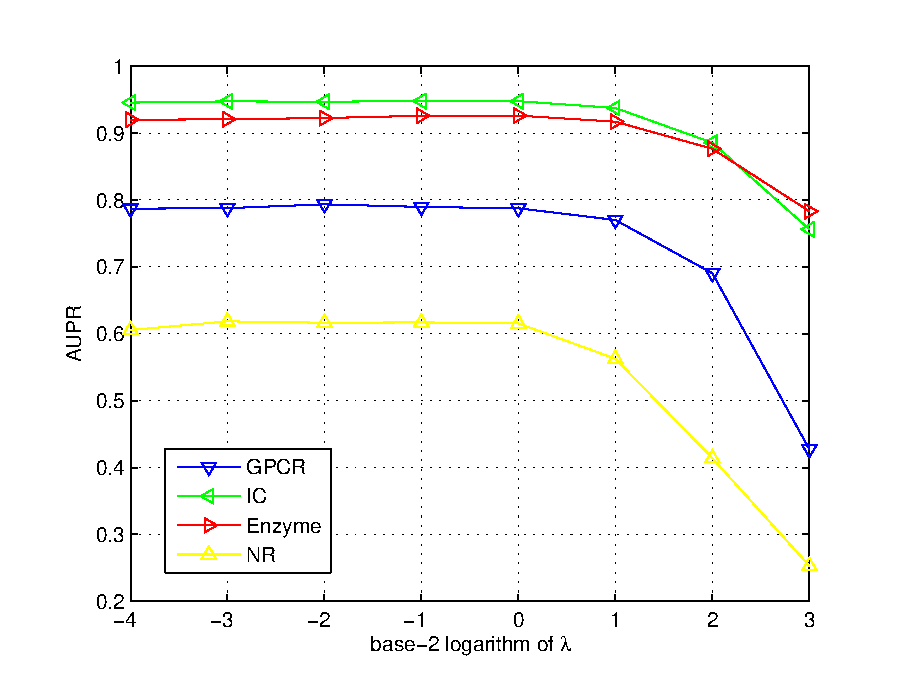
\includegraphics[width=8cm]{effect_lambda}
\caption{The effect of parameter $\lambda$}\label{effect_lambda}
\end{figure}
\begin{figure} [htbp]
\centering
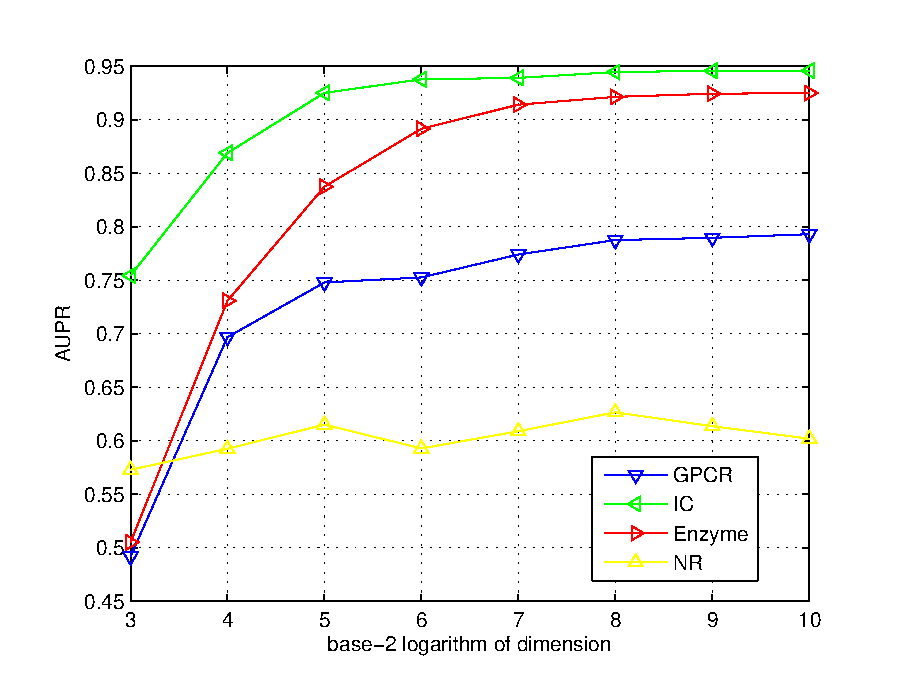
\includegraphics[width=8cm]{effect_dim}
\caption{The effect of dimensions.}\label{effect_dim}
The dimensionality is increased from 8 to 1024.
\end{figure}

\section{Conclusion}
In this paper, we proposed two new methods (MSTMF and MSTMF-weight) to model multiple similarities for drug target interaction prediction. And we experimently improved that our methods achieved significantly better performance than any other methods using AUPR as a criteria. In addition, our proposed method MSTMF has only one parameter $\lambda$, and the prediction result is quite stable with respect to its parameter. This is a big advantage which MSCMF doesn't have.    \\

\section{Acknowledgments}
This is Acknowledgments.

%% The file named.bst is a bibliography style file for BibTeX 0.99c
\bibliographystyle{ijcai15}
\bibliography{ref}

\end{document}

